% =============================================================================
%  aaddrick/claude-desktop-debian -- Official Claude Desktop for Linux teardown
%  Report CDL-ANT-0008. Built on the NCL LaTeX report template (XeLaTeX).
%  House style: no em dashes; en dashes only for numeric ranges.
% =============================================================================
\nonstopmode
\documentclass[11pt]{article}
\usepackage[letterpaper,top=13mm,bottom=16mm,left=13mm,right=13mm,footskip=9mm]{geometry}
\usepackage{fontspec}
\usepackage[table,dvipsnames]{xcolor}
\usepackage{array}
\usepackage{tikz}
\usetikzlibrary{shadings,fadings,positioning,arrows.meta}
\usepackage{eso-pic}
\usepackage{graphicx}
\usepackage{float}
\usepackage{booktabs}
\usepackage{titlesec}
\usepackage{enumitem}
\usepackage{microtype}
\usepackage{fancyvrb}
\usepackage[hidelinks]{hyperref}
\usepackage{parskip}
\usepackage{fancyhdr}

% ---- Graphite + Copper palette ----
\definecolor{base900}{HTML}{1A1B1E}
\definecolor{base800}{HTML}{24262A}
\definecolor{base700}{HTML}{30343A}
\definecolor{base600}{HTML}{3A3D44}
\definecolor{baseMid}{HTML}{5C616A}
\definecolor{ink}{HTML}{181B20}
\definecolor{muted}{HTML}{43505D}
\definecolor{faint}{HTML}{6B7480}
\definecolor{line}{HTML}{E2E4E8}
\definecolor{linestrong}{HTML}{CDD0D6}
\definecolor{paperalt}{HTML}{F5F6F8}
\definecolor{accent}{HTML}{B05B33}
\definecolor{accentsoft}{HTML}{E2B89C}
\definecolor{accentbg}{HTML}{FAF1EA}
\definecolor{accentink}{HTML}{7C3E20}

% ---- fonts ----
\setmainfont{Public Sans}[
  UprightFont={* Regular}, BoldFont={* Bold},
  ItalicFont={* Italic}, BoldItalicFont={* Bold Italic}]
\newfontfamily\heavy{Public Sans}[UprightFont={* ExtraBold}]
\setmonofont{IBM Plex Mono}[Scale=0.92,
  UprightFont={* Regular}, BoldFont={* SemiBold}]
\newfontfamily\symfont{DejaVu Sans}
\newcommand{\mono}{\ttfamily}
\newcommand{\arrow}{{\symfont\char"2192}}

\setlength{\parindent}{0pt}
\setlength{\parskip}{0pt}
\linespread{1.12}
\color{ink}

% ---- body paragraph ----
\newcommand{\reppar}[1]{{\fontsize{10.5}{15.2}\selectfont #1\par}\vspace{8pt}}
% inline code (escape _, &, %, #, $, ~, ^ manually in the argument)
\newcommand{\code}[1]{{\mono\small #1}}

% ---- mono eyebrow ----
\newcommand{\eyebrow}[1]{{\mono\footnotesize\color{baseMid}\addfontfeatures{LetterSpace=8.0}\MakeUppercase{#1}}}

% ---- section header ----
\newcommand{\reportsection}[3]{%
  \vspace{14pt}%
  {\mono\footnotesize\color{baseMid}\addfontfeatures{LetterSpace=8.0}\MakeUppercase{#1\, \textbullet\, #2}}\par
  \vspace{3pt}%
  {\heavy\fontsize{17}{19}\selectfont\color{base900} #3\par}
  \vspace{4pt}{\color{accent}\hrule height 1.6pt}\vspace{9pt}%
}

% ---- figure caption ----
\newcommand{\figcap}[1]{\par\vspace{4pt}%
  {\color{faint}\fontsize{8.5}{11}\selectfont #1\par}}

% ---- table helpers ----
\newcommand{\tabcap}[1]{{\mono\color{faint}\fontsize{8.4}{11}\selectfont #1\par}\vspace{5pt}}
\newcommand{\thd}[1]{{\mono\bfseries\footnotesize\color{white}\MakeUppercase{#1}}}
\newcommand{\thdr}[1]{\multicolumn{1}{r}{\thd{#1}}}
\newcommand{\tname}[1]{\textbf{\color{base700}#1}}
\newcommand{\pct}[1]{{\mono\color{faint}\small #1}}

% ---- copper method-note banner ----
\newcommand{\methodbanner}[1]{%
  \begingroup\setlength{\fboxsep}{11pt}%
  \noindent\fcolorbox{accentsoft}{accentbg}{%
    \parbox{\dimexpr\linewidth-2\fboxsep-2\fboxrule}{%
      \color{accentink}\fontsize{9.4}{13.5}\selectfont #1}}\par\endgroup\vspace{8pt}}

% ---- code block (copper left rule, Plex Mono) ----
\DefineVerbatimEnvironment{codeblock}{Verbatim}%
  {fontsize=\footnotesize,frame=leftline,framerule=1.4pt,%
   rulecolor=\color{accent},framesep=9pt,xleftmargin=2pt,%
   formatcom=\color{base700}}

% ---- convergence badge ----
\newcommand{\badge}[2]{{\mono\bfseries\fontsize{7.4}{8}\selectfont\colorbox{#1}{\color{white}\,\MakeUppercase{#2}\,}}}
\newcommand{\bsame}{\badge{base700}{converge}}
\newcommand{\bdiff}{\badge{accent}{diverge}}
\newcommand{\bofc}{\badge{base600}{official only}}
\newcommand{\bcom}{\badge{baseMid}{community only}}

% ---- title-block key label ----
\newcommand{\kvk}[1]{{\mono\bfseries\footnotesize\color{base700}\MakeUppercase{#1}}}

% ---- running footer ----
\fancypagestyle{reportftr}{%
  \fancyhf{}%
  \renewcommand{\headrulewidth}{0pt}%
  \renewcommand{\footrulewidth}{0pt}%
  \fancyfoot[C]{\parbox{\linewidth}{%
    {\color{linestrong}\hrule}\vspace{4pt}%
    {\mono\color{faint}\fontsize{7.6}{10}\selectfont CDL-ANT-0008 \textperiodcentered{} Official Claude Desktop for Linux Teardown \hfill aaddrick/claude-desktop-debian \textperiodcentered{} July 1, 2026 \textperiodcentered{} p.\,\thepage}%
  }}%
}

\begin{document}
\pagestyle{reportftr}
% Prefer occasional loose lines over long inline-code tokens bleeding past the
% right margin: let the breaker put an unbreakable \code{} token on a fresh line.
\sloppy
\emergencystretch=2.5em
\hbadness=3000

% ===== COVER =====
\AddToShipoutPictureBG*{%
  \AtPageLowerLeft{%
    \begin{tikzpicture}[remember picture,overlay]
      \shade[top color=base900, bottom color=base700, middle color=base800]
        (current page.north west)
        rectangle ([yshift=-150mm]current page.north east);
      \begin{scope}
        \clip (current page.north west) rectangle ([yshift=-150mm]current page.north east);
        \shade[inner color=accent, outer color=base900, opacity=0.18]
          ([xshift=-14mm,yshift=8mm]current page.north east) circle (62mm);
      \end{scope}
    \end{tikzpicture}}}
\thispagestyle{reportftr}
\vspace*{26mm}
{\color{white}%
  {\heavy\fontsize{20}{22}\selectfont aaddrick/claude-desktop-debian}\par
  \vspace{24mm}
  {\mono\footnotesize\addfontfeatures{LetterSpace=11.0}\textcolor{white!82}{SOFTWARE TEARDOWN / BINARY ANALYSIS}}\par
  \vspace{10pt}
  {\heavy\fontsize{33}{36}\selectfont Inside the Official \\[2pt] Claude Desktop for Linux\par}
  \vspace{11pt}
  {\fontsize{13}{18}\selectfont\textcolor{white!88}{\parbox{135mm}{What Anthropic actually implemented on the Linux code paths of the 1.17377.1 beta, verified against the shipped bytes, and how it compares to the community repackage.}}\par}
}
\vspace*{0pt}\vspace{22mm}

\renewcommand{\arraystretch}{1.6}\setlength{\tabcolsep}{10pt}
\noindent\begin{tabular}{@{}>{\columncolor{paperalt}}m{32mm} m{\dimexpr\linewidth-32mm-2\tabcolsep-2\arrayrulewidth\relax}@{}}
\hline
\kvk{Document} & CDL-ANT-0008 \textperiodcentered{} Rev A \textperiodcentered{} FINAL \\ \hline
\kvk{Subject} & Teardown of the official Claude Desktop for Linux beta \\ \hline
\kvk{Focus} & What ships in the Linux code paths, and where it converges with or diverges from the community repackage \\ \hline
\kvk{Scope} & \code{claude-desktop\_1.17377.1\_amd64.deb} (Electron 42.5.1), pulled from the official APT pool 2026-06-30; cross-referenced against \code{aaddrick/claude-desktop-debian} \\ \hline
\kvk{Tools} & \code{dpkg-deb}, \code{@electron/asar}, \code{prettier}, \code{grep}/\code{strings}, and a 22-agent teardown workflow with adversarial byte-level verification \\ \hline
\kvk{Headline} & The official build is a genuine first-party native port that independently reaches many of the community's Linux fixes, while adding capabilities a repackage cannot. \\ \hline
\kvk{Author} & Claude Opus 4.8 \textperiodcentered{} July 1, 2026 \\ \hline
\kvk{Reviewed by} & Aaddrick Williams \\ \hline
\end{tabular}
\clearpage

% ===== BODY =====

\reportsection{01}{Overview}{The Official Build Is Real, and It Agrees With You}

\reppar{On June 30, 2026, Anthropic shipped the first-party \textbf{Claude Desktop for Linux} beta: Ubuntu 22.04+ and Debian 12+, x86\_64 and arm64, delivered through an official APT repository, carrying the full \textbf{Chat, Cowork, and Code} tab set. This report tears down the actual artifact, \code{claude-desktop\_1.17377.1\_amd64.deb}, and reads what Anthropic wrote for Linux out of the shipped bytes. \textbf{1.17377.1 is the exact upstream build that \code{claude-desktop-debian} already tracks}, so the comparison between the official port and the community repackage is like-for-like.}

\reppar{The headline finding is twofold. First, on the fixes that a repackage was forced to inject, \textbf{the official build independently converges on the same answers}: an in-place tray icon update that sidesteps the KDE duplicate-icon race, a SUID sandbox helper paired with an AppArmor \code{userns} profile for Ubuntu 24.04+, an Electron \code{globalShortcut} registration merged with the Wayland \code{GlobalShortcutsPortal} feature flag, and a self-updater that is disabled at the source. Second, it ships \textbf{native capability a repackage structurally cannot}: a real KVM/QEMU Cowork virtual machine, a Rust native binding that performs genuine X11 input injection for computer use, a Rust browser native-messaging host, and a first-party signed APT channel.}

\reppar{The practical consequence for the community project is a shift in its center of gravity rather than obsolescence. Several of its most intricate patches are now redundant \emph{against the official Debian package}, while its real remaining value moves to the distributions and environments Anthropic does not serve: Fedora and RPM, AppImage, NixOS, Arch, and hosts without KVM or with native Wayland. The rest of this report walks each subsystem, then closes with a convergence matrix and the strategic implications.}

\methodbanner{\textbf{Method and provenance.} The \code{.deb} was pulled from \code{downloads.claude.ai/claude-desktop/apt/stable} (SHA-256 \code{f4bd785\ldots c85c7}), unpacked with \code{dpkg-deb}, and its \code{app.asar} extracted and beautified. Every claim below is grounded in a file path and, where useful, a line reference in the beautified \code{index.js} / \code{index.pre.js} or in \code{strings} output from a shipped binary. Findings were produced by parallel per-subsystem agents and then re-checked by an adversarial verifier against the same bytes; the load-bearing facts (launch switches, sandbox bit, updater kill, Cowork download, native-binding symbols) were additionally confirmed by hand. Claims about the community side rest on reads of \code{scripts/patches/*.sh} and \code{docs/learnings/*.md}.}

\reportsection{02}{Inventory}{What Is in the Package}

\reppar{The package installs a conventional \code{electron-forge} tree under \code{/usr/lib/claude-desktop} with the launcher symlinked to \code{/usr/bin/claude-desktop}, but the interesting mass is the set of Linux-native helper binaries and VM assets in \code{resources/}. Three of them are compiled programs written specifically for this port: a Go daemon that runs the Cowork VM, a Rust virtio-fs daemon, and a Rust bridge to browser extensions. The build is Electron \textbf{42.5.1} (the \code{version} file reads \code{42.5.1}) and the app declares \code{node >= 22}.}

\begin{table}[H]
\tabcap{Linux-native artifacts shipped in the .deb. Sizes are on-disk; language inferred from build strings.}
\setlength{\tabcolsep}{7pt}\renewcommand{\arraystretch}{1.3}
\rowcolors{3}{paperalt}{white}
\noindent\begin{tabular}{@{}l r l >{\raggedright\arraybackslash}p{88mm}@{}}
\rowcolor{base800}
\thd{Artifact} & \thdr{Size} & \thd{Kind} & \multicolumn{1}{l}{\thd{Role on Linux}} \\
\tname{claude-desktop} & 207\,MiB & ELF (Electron) & Main app binary; launcher symlink target. \\
\tname{chrome-sandbox} & 15\,KB & ELF, SUID 4755 & Chromium setuid sandbox helper. \\
\tname{chrome\_crashpad\_handler} & 1.9\,MB & ELF & Out-of-process crash capture. \\
\tname{cowork-linux-helper} & 3.1\,MB & Go, static & \code{coworkd}: boots and supervises the Cowork QEMU VM. \\
\tname{virtiofsd} & 2.6\,MB & Rust & virtio-fs host daemon shared into the VM. \\
\tname{chrome-native-host} & 1.1\,MB & Rust & Chrome native-messaging \arrow{} MCP bridge. \\
\tname{claude-native-binding.node} & 1.65\,MB & Rust NAPI & Native addon: X11 input injection, XDG/MIME, safe-fs. \\
\tname{smol-bin.x64.img} & 24\,MB & disk image & Auxiliary virtio-blk disk for the VM. \\
\tname{node-pty (linux-x64)} & prebuilt & native & Pseudo-terminal for Code/agent shells. \\
\tname{TrayIconLinux(-Dark).png} & 64$\times$64 & PNG & Purpose-made Linux tray icons. \\
\end{tabular}
\end{table}

\reppar{The \code{Depends} line is a precise map of the runtime contract: \code{libgtk-3-0}, \code{libnotify4}, \code{libnss3}, \code{libsecret-1-0}, \code{libatspi2.0-0}, \code{libdrm2}, \code{libgbm1}, \code{xdg-utils}, a hard \code{xdg-desktop-portal} plus a GTK/GNOME/KDE portal backend, and a trash provider (\code{kde-cli-tools} \code{|} \code{trash-cli} \code{|} \code{gvfs}, among others). \code{Recommends} adds the tray and secret backends (\code{libayatana-appindicator3-1} \code{|} \code{libappindicator3-1}; \code{gnome-keyring} \code{|} \code{kwalletd6} \code{|} \code{kwalletd5}) and \textbf{\code{qemu-system-x86}, \code{ovmf}, and \code{virtiofsd}}: the Cowork VM stack. The \code{.desktop} entry registers the \code{claude://} URL scheme with two quick actions (New chat, New Claude Code session) and sets \code{SingleMainWindow=true} so GNOME suppresses a spurious "New Window" item.}

\reportsection{03}{Sandbox}{SUID Helper, AppArmor userns, and Four Switches}

\reppar{The entry point is \code{.vite/build/index.pre.js} (per \code{package.json} \code{main}), and it is deliberately restrained about Chromium command-line switches. It appends exactly four, and no more: \code{disable-logging} (when packaged and \code{CLAUDE\_ENABLE\_LOGGING} is unset), \code{enable-features=DocumentPolicyIncludeJSCallStacksInCrashReports}, \code{enable-features=\ldots,GlobalShortcutsPortal}, and, on one specific KDE path, \code{password-store=basic}. It does \textbf{not} append \code{--no-sandbox}, \code{--disable-gpu}, or \code{--ozone-platform}. The sandbox stays on and hardware acceleration is left to Chromium's own decision. Only an in-app setting toggles hardware acceleration.}

\reppar{Sandboxing is handled the way Chrome, VS Code, and 1Password handle it. The \code{chrome-sandbox} helper ships \textbf{SUID root, mode 4755} (verified: \code{-rwsr-xr-x}), and the \code{postinst} writes an AppArmor profile so Chromium's user-namespace sandbox works on Ubuntu 24.04+, where \code{kernel.apparmor\_restrict\_unprivileged\_userns=1} otherwise blocks \code{CLONE\_NEWUSER} for unconfined processes. The profile is not confinement; \code{flags=(unconfined)} only allowlists the binary for \code{userns}:}

\begin{codeblock}
abi <abi/4.0>,
include <tunables/global>

profile claude-desktop /usr/lib/claude-desktop/claude-desktop flags=(unconfined) {
  userns,
  include if exists <local/claude-desktop>
}
\end{codeblock}

\reppar{The profile is gated on the presence of \code{/etc/apparmor.d/abi/4.0}, which only ships with AppArmor 4.0, so on Ubuntu 22.04 / Debian 12 (AppArmor 3.x) it is skipped and the SUID helper carries the load. Crash reporting is wired through \code{crashReporter.start(\{uploadToServer:false\})} with the \code{chrome\_crashpad\_handler} binary capturing minidumps locally, which are then annotated and forwarded to Sentry.}

\methodbanner{\textbf{Community parity.} This is the same design \code{claude-desktop-debian} already uses: a 4755 \code{chrome-sandbox} and an unconfined \code{userns} AppArmor profile. The community launcher goes further where a repackage must: it injects \code{--no-sandbox} for the AppImage (FUSE) and Wayland-deb cases, flips \code{--ozone-platform=wayland} under \code{CLAUDE\_USE\_WAYLAND=1}, and adds a GPU-crash auto-recovery path (\code{--disable-gpu --disable-software-rasterizer} after a fatal GPU process exit). The official build has no ozone flip and no GPU auto-recovery; it records \code{gpu\_compositing} telemetry and exposes a manual toggle instead.}

\reportsection{04}{Tray}{The AppIndicator Path, Done Natively}

\reppar{The tray is a stock Electron \code{Tray} instance (\code{new Tray(nativeImage.createFromPath(t))}), which on Linux binds to the AppIndicator / StatusNotifierItem stack; the \code{libayatana-appindicator3-1} recommendation confirms it. There is no left-click handler anywhere, which is correct for SNI, where activation is menu-only; the "Show App" menu item does the show/restore/focus. Anthropic ships \textbf{dedicated 64$\times$64 Linux icons}, \code{TrayIconLinux.png} and \code{TrayIconLinux-Dark.png}, selected through a genuine platform constant (\code{uKr = "png"}), and picks the light-on-dark icon when the desktop is GNOME \emph{or} \code{nativeTheme.shouldUseDarkColors} is true. The desktop environment is read from \code{XDG\_CURRENT\_DESKTOP} with a \code{KDE\_FULL\_SESSION} fallback.}

\reppar{The official build \textbf{never opens the KDE duplicate-icon window in the first place}. On a \code{nativeTheme "updated"} event, the rebuild takes an in-place branch: it calls \code{Tray.setImage(\ldots)} only when the resolved icon path actually changed, and returns. \code{Tray.destroy()} is called on exactly one path: when the user disables the tray. Because a theme change never destroys and recreates the \code{StatusNotifierItem}, the unregister/register gap that briefly shows two icons on Plasma's system tray never exists. The menu is updated on a separate path guarded by a serialized-fingerprint diff (skipping redundant DBus \code{LayoutUpdated} emissions) with a 32-entry strong-reference retention buffer for superseded menu objects.}

\methodbanner{\textbf{Community parity.} This is precisely the outcome \code{patch\_tray\_inplace\_update} chases in \code{tray.sh}: inject a \code{setImage} guard ahead of upstream's destroy-and-recreate. The difference is that the community patch also needs a 250ms post-destroy delay and a trailing-edge mutex (issue \#679) because its starting point still contains the destroy path; the official design removes the need for both. See \code{docs/learnings/tray-rebuild-race.md}: the learning stays accurate for the repackage, but should note that the official build solves this natively. The community also has no purpose-made Linux icon (it retargets the 24$\times$24 macOS template icon) and no GNOME special-case.}

\reportsection{05}{Cowork}{A Real KVM Virtual Machine, Booted by a Go Daemon}

\reppar{Cowork on Linux is the single largest piece of net-new engineering, and it is a real virtual machine, not a container. The \code{cowork-linux-helper} binary is a statically linked Go program (\code{coworkd}) whose strings expose its structure directly: \code{coworkd/\allowbreak cmd/\allowbreak cowork-linux-helper/\allowbreak\{main,vm,server,guestrpc,protocol\}.go}. Electron talks to it over a Unix socket with \textbf{\code{SO\_PEERCRED} peer verification}, and \code{coworkd} launches QEMU on the \code{q35} machine with OVMF firmware (\code{FirmwareCodePath} plus a per-boot writable EFI vars template), a \code{virtiofsd} share (tag \code{claudeshared}), and a \code{vhost-vsock} channel over which the guest RPC runs with CID validation. QEMU itself runs under a seccomp sandbox: \code{obsolete=deny,\allowbreak elevateprivileges=deny,\allowbreak spawn=deny,\allowbreak resourcecontrol=deny}.}

\begin{figure}[H]\centering
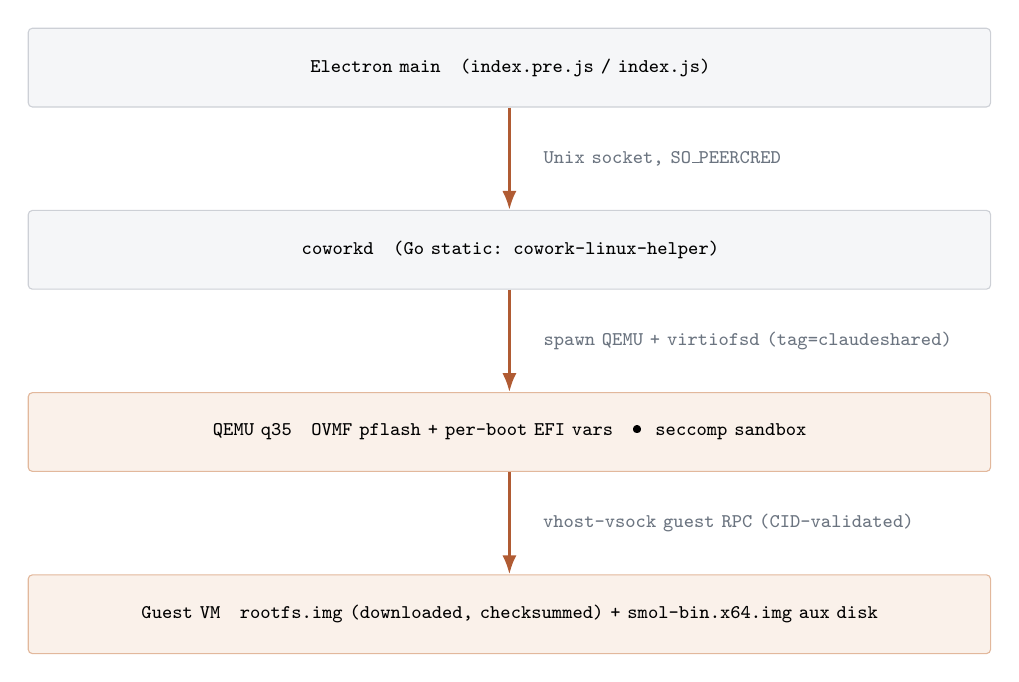
\begin{tikzpicture}[
  font=\mono\scriptsize,
  box/.style={draw=linestrong, fill=paperalt, rounded corners=1.5pt, align=center,
              inner sep=6pt, minimum height=10mm, text width=118mm},
  vmbox/.style={draw=accentsoft, fill=accentbg, rounded corners=1.5pt, align=center,
              inner sep=6pt, minimum height=10mm, text width=118mm},
  ar/.style={-{Latex[length=2.4mm]}, draw=accent, line width=1pt},
  lbl/.style={font=\mono\scriptsize, color=faint, align=left, text width=54mm}
]
\node[box] (el) {\textbf{Electron main} \; (index.pre.js / index.js)};
\node[box, below=13mm of el] (cd) {\textbf{coworkd} \; (Go static: cowork-linux-helper)};
\node[vmbox, below=13mm of cd] (qemu) {\textbf{QEMU q35} \; OVMF pflash + per-boot EFI vars \; \textbullet\; seccomp sandbox};
\node[vmbox, below=13mm of qemu] (guest) {\textbf{Guest VM} \; rootfs.img (downloaded, checksummed) + smol-bin.x64.img aux disk};
\draw[ar] (el) -- (cd) node[lbl, midway, right=3mm]{Unix socket, SO\_PEERCRED};
\draw[ar] (cd) -- (qemu) node[lbl, midway, right=3mm]{spawn QEMU + virtiofsd (tag=claudeshared)};
\draw[ar] (qemu) -- (guest) node[lbl, midway, right=3mm]{vhost-vsock guest RPC (CID-validated)};
\end{tikzpicture}
\figcap{The Cowork boot chain on Linux. Copper boxes run inside the virtualization boundary. The rootfs is fetched at runtime, not shipped in the .deb; the bundled smol-bin image is a secondary virtio-blk disk.}
\end{figure}

\reppar{One correction to the intuitive reading: the Linux VM downloads part of itself at runtime. The boot rootfs is fetched from \code{downloads.claude.ai/vms/linux/\$\{arch\}/\$\{sha\}/\$\{file\}} (a checksummed \code{rootfs.img}, alongside \code{condadata.img} and \code{sessiondata.img}); the 24\,MB \code{smol-bin.x64.img} bundled in the package is a separate auxiliary disk (\code{drive=smolbindisk}), not the rootfs. The \code{virtiofsd} selection prefers a system binary and falls back to the bundled one only on Ubuntu 22.x; on other distros without a system \code{virtiofsd} the feature is reported as APT-installable rather than silently degraded.}

\methodbanner{\textbf{Community divergence.} \code{cowork.sh} reroutes Cowork to a hand-written Node.js daemon whose default backend is \code{bwrap} (bubblewrap), running the workload host-direct with an optional opt-in KVM path via \code{COWORK\_VM\_BACKEND}; it deliberately disables the multi-gigabyte rootfs download and ships a second AppArmor profile for \code{/usr/bin/bwrap}. There is no \code{vsock}, no QEMU seccomp, and no \code{SO\_PEERCRED}. The two approaches optimize opposite constraints: the official build wants a strong VM boundary and accepts a hard \code{/dev/kvm} + \code{vhost\_vsock} + OVMF requirement; the community build wants Cowork to run at all on hosts without nested virtualization. See \code{docs/learnings/cowork-vm-daemon.md}.}

\reportsection{06}{Window}{A System Frame, and No Topbar Shim}

\reppar{The official Linux window is a plain system-decorated window. The main \code{BrowserWindow} omits \code{frame}, so it defaults to \code{frame:true} and the window manager draws the titlebar; \code{titleBarStyle} and \code{titleBarOverlay} are macOS/Windows concerns and are inert here (the \code{setTitleBarOverlay} call is wrapped in a try/catch commented as "probably expected" to fail). The app also \textbf{does not spoof the user agent}. Because claude.ai only renders its in-app Windows-style topbar when it detects a Windows client, that topbar simply never appears on Linux, and the app relies on the system frame plus claude.ai's default web chrome.}

\methodbanner{\textbf{Community divergence.} The repackaged Windows bundle ships \code{frame:false}, which on X11 produces unclickable window-control buttons because of a Chromium-level implicit drag region. \code{frame-fix-wrapper.js} forces \code{frame:true}, and the community's "hybrid mode" (\code{wco-shim.sh}) appends \code{" Windows"} to the UA so claude.ai renders its topbar in a stacked layout with working buttons. The shim exposes several \code{CLAUDE\_TITLEBAR\_STYLE} modes. The official build sidesteps the entire problem by never going frameless and never spoofing the UA. See \code{docs/learnings/linux-topbar-shim.md}, which should be annotated to record that the official build ships the system-frame path.}

\reportsection{07}{Shortcuts}{Global Hotkey, Autostart, and the Wayland Gap}

\reppar{Quick Entry's global hotkey is registered through Electron's \code{globalShortcut.register()} (default \code{Ctrl+Alt+Space}), and the app does two Linux-aware things around it. It merges \code{GlobalShortcutsPortal} into \code{--enable-features} with a read-then-append discipline (so it does not clobber an existing \code{--enable-features} value), and at runtime it probes the portal over \code{busctl}, gates on X11 vs Wayland, and surfaces an \code{unsupported\_session} status in-app when the session cannot support the hotkey. Toggling the feature writes an XDG autostart \code{.desktop} entry (the \code{postrm} explicitly leaves \code{~/.config/autostart} residue in place, since maintainer scripts must not reach into user homes).}

\reppar{The gap is the same one the community documented. The launcher ships a bare ELF and a plain \code{.desktop}, so the app \textbf{defaults to XWayland}, where the \code{GlobalShortcutsPortal} feature flag is inert: the portal only matters under native Wayland (Ozone), which the official build never enables. Anthropic wired the portal but did not flip the switch that would make the app talk to it by default.}

\methodbanner{\textbf{Community parity, with an escape hatch.} \code{claude-desktop-debian} uses the same \code{globalShortcut} API and the same \code{--enable-features} merge discipline, but its launcher flips \code{--ozone-platform=wayland} (opt-in via \code{CLAUDE\_USE\_WAYLAND=1}, tri-state) so the portal is actually reachable on native Wayland. The XDG autostart write is upstream app code the repackage cannot itself add. The learning in \code{docs/learnings/wayland-global-shortcuts-portal.md}, including the GNOME 50 / \code{electron\#51875} host-handshake blocker, applies verbatim to the official build and is now directly filable upstream.}

\reportsection{08}{Secrets}{os\_crypt, a KWallet Preflight, and the Refusal to Persist Insecurely}

\reppar{Secret storage leans on Chromium's \code{os\_crypt} auto-detection (libsecret or KWallet), but adds a KDE-specific safety valve. At launch, when the desktop is KDE and no \code{--password-store} is explicitly set, the app runs a \code{busctl --user} preflight against \code{org.kde.kwalletd6} / \code{kwalletd5} to detect the "reachable but no wallet yet" state. If it sees that state, it forces \code{--password-store=basic} so that Chromium's cookie-encryption init cannot wedge the network service behind KWallet's blocking wallet-creation dialog. The same probe runs again at runtime and warns that a later \code{safeStorage} call would otherwise "freeze this thread behind the wallet-creation wizard".}

\reppar{Where no encryption backend is available at all, the official build makes a deliberate choice: it \textbf{declines to persist} OAuth, MCP, and pairing tokens rather than writing them weakly, and shows a one-time "install or unlock a keyring" notice (gated on \code{!CI}) plus telemetry. Roughly 35 code sites guard on \code{safeStorage.isEncryptionAvailable()} out of about 70 total \code{safeStorage} touch-points.}

\methodbanner{\textbf{Community divergence.} The community launcher's \code{\_detect\_password\_store} always forces a backend (\code{kwallet6} / \code{gnome-libsecret} / a fixed-key \code{basic} fallback), so tokens always persist even with no keyring, and it surfaces the chosen backend in \code{doctor.sh}. The official build prioritizes "do not persist insecurely"; the community build prioritizes "always persist, even if only filesystem-permission protected." For headless or kiosk users the community behavior is more convenient; for the default desktop the official behavior is safer.}

\reportsection{09}{Native binding}{Real X11 Computer Use, Written in Rust}

\reppar{On Linux, the \code{@ant/claude-native} addon is a real 1.65\,MB NAPI-RS Rust binding, not a stub. Its symbols show genuine capability: \code{enigo} and \code{x11rb} (with \code{XTEST}) for X11 input injection, which is what backs computer use; \code{rustix} with \code{openat2} for safe-filesystem containment; and \code{SO\_PEERCRED} for socket peer authentication. This is a first-party, platform-native implementation of the input and filesystem primitives rather than an Electron-level approximation. Hardware-backed keys and web authentication are explicitly marked "not yet supported" on Linux.}

\methodbanner{\textbf{Community divergence.} A repackage cannot run the Windows \code{.node}, so \code{claude-desktop-debian} replaces it with \code{claude-native-stub.js}: \code{KeyboardKey} constants, \code{flashFrame} / \code{getIsMaximized} via Electron's \code{BrowserWindow}, \code{AuthRequest.isAvailable()} hardwired to false, and no-ops for the Windows registry and MSIX paths. Real input injection and peer-cred sockets are approximated or dropped. This is the one capability the official build has that the community build cannot reproduce without reimplementing a Rust addon.}

\reportsection{10}{Browser and links}{A Native-Messaging Host, and Protocol Handling}

\reppar{The official build ships \textbf{"Claude in Chrome" plumbing} that the community package lacks entirely. \code{chrome-native-host} is a Rust binary that bridges Chrome's native-messaging protocol to MCP (its strings include \code{claude-mcp-browser-bridge-}, \code{native\_host\_version 0.1.0}, and \code{ToolRequest}), and the app auto-installs and removes a \code{com.anthropic.claude\_browser\_extension.json} manifest into the Chrome/Edge \code{NativeMessagingHosts} directories. A filesystem watcher tracks it. Deep links are registered with \code{setAsDefaultProtocolClient("claude")} plus the \code{.desktop} \code{MimeType} and two Desktop Actions, and a single \code{disableDeepLinkRegistration} setting is the kill-switch for both OS registration and incoming-link handling. File dialogs are portal-aware (the hard \code{xdg-desktop-portal} dependency), and trash is delegated to a packaged trash provider.}

\methodbanner{\textbf{Community divergence.} The repackage has no native-messaging host and no browser bridge at all; \code{claude://} is registered via the \code{.desktop} \code{MimeType} only, with no Desktop Actions, and AppImage login is deferred to a third-party tool. The community \code{.deb} also assumes the portal and trash providers are present rather than declaring them as dependencies.}

\reportsection{11}{MCP and PATH}{Login-Shell Environment, and a Bug That Survived}

\reppar{The official build solves a problem the community repackage does not even attempt: recovering the user's real interactive environment. It forks a \code{utilityProcess} (\code{shellPathWorker.js}) that runs \code{\$SHELL -l -i -c} to dump the login-shell PATH and environment, merges it with a hardcoded toolchain and NixOS \code{bin} directory list and \code{process.env}, and hands the result to the Code sessions and MCP subprocesses. System proxy settings are resolved via \code{session.resolveProxy()} and exported as \code{HTTPS\_PROXY} / \code{HTTP\_PROXY} / \code{NO\_PROXY} into those subprocesses. Stdio MCP servers are spawned through the Agent SDK's \code{StdioClientTransport} over \code{cross-spawn} with \code{shell:false}.}

\reppar{The \textbf{stdio double-spawn bug documented by the community is present and unfixed in the official 1.17377.1 build}: when a chat coordinator and the Code/Agent coordinator are both active, a stdio MCP server is launched twice. The community learning correctly characterized this as an upstream defect, not a repackaging artifact, and this teardown confirms it against first-party code.}

\methodbanner{\textbf{Implication.} \code{docs/learnings/mcp-double-spawn.md} is now validated against the official build. This is a clean upstream bug report to file against a first-party Linux target, where a fix reaches every Linux user rather than only the repackage.}

\reportsection{12}{Quieter surfaces}{Detection, Telemetry, and the Small Linux Touches}

\reppar{Beyond the headline subsystems, the build carries a Linux-only detection and telemetry layer with no analog in the repackage. It reads \code{/etc/os-release} (falling back to \code{/usr/lib/os-release}) for \code{ID} and \code{VERSION\_ID}, classifies the session type against \code{\{x11, wayland, tty, mir\}}, resolves the desktop environment, and reports all four as Sentry tags (\code{linux\_distro}, \code{linux\_distro\_version}, \code{linux\_session\_type}, \code{linux\_desktop\_environment}). Hardware-acceleration state is bucketed into \code{gpu\_compositing} telemetry, and a \code{--disable-gpu} switch is recognized as its own bucket.}

\reppar{The remaining Linux touches are unremarkable but correct: native notifications via \code{libnotify} carry an \code{urgency} field (low / normal / critical) and action buttons, with only \code{subtitle} and \code{hasReply} macOS-gated; \code{powerSaveBlocker} provides refcounted keep-awake and \code{powerMonitor} pauses the renderer watchdog on suspend/lock; a single-instance lock forwards second-instance argv (de-duplicated) and routes \code{.dxt} / \code{.mcpb} files to the extension installer and everything else to the URL handler; \code{SIGINT}/\code{SIGTERM}/\code{SIGQUIT}/\code{SIGHUP} trigger a clean quit; and spellcheck uses Chromium's hunspell with an add-to-dictionary context menu. Screen capture through \code{desktopCapturer} depends on the portal's ScreenCast backend under Wayland, and a "wayland resize race" guard resyncs stale view bounds on focus.}

\reportsection{13}{Auto-update}{Turned Off at the Source}

\reppar{The Linux build does not self-update, and it says so plainly. The updater bootstrap early-returns with the log line \code{[updater] Linux: in-app updater off (apt channel not yet live)} and a telemetry reason of \code{apt\_channel\_pending}; the feed-URL and \code{checkForUpdates} machinery still exists in the bundle but is unreachable on a normal install, and "Check for updates" opens the browser. Updates are expected to arrive through the package manager once the APT channel goes live.}

\reppar{The distribution design behind that is visible in the maintainer scripts. The \code{postinst} always writes the Anthropic signing key (RSA-4096, fingerprint \code{31DD DE24 DDFA B679 F42D 7BD2 BAA9 29FF 1A7E CACE}) and self-registers the APT repository at \code{downloads.claude.ai/claude-desktop/apt/stable} on the VS Code / Chrome / 1Password model, but currently ships the \code{deb} line \textbf{commented out} (\code{APT\_REPO\_DEFAULT="false"}) until the channel is published, toggled by \code{CLAUDE\_DESKTOP\_ADD\_REPO} in \code{/etc/default/claude-desktop}. The scripts are \code{DPKG\_ROOT}-aware for chrootless installs, defend against symlink attacks, and parse the defaults file rather than sourcing it (so target-rootfs content cannot execute as host root).}

\methodbanner{\textbf{Community parity, different mechanism.} The community reaches the same end-state (no self-update) by intercepting \code{require('electron')} in \code{frame-fix-wrapper.js} and swapping \code{autoUpdater} for a no-op Proxy (issue \#567), because the repackaged Windows bundle carries a live feed URL. Its distribution is a Cloudflare Worker fronting \code{gh-pages} that 302-redirects binaries to GitHub Release assets (to dodge GitHub's 100\,MB push cap), across \code{.deb} + \code{.rpm} + AppImage + Nix. See \code{docs/learnings/apt-worker-architecture.md}.}

\reportsection{14}{Comparison}{Official Port vs Community Repackage}

\reppar{The matrix below reduces the teardown to one row per dimension. "Converge" means both arrive at the same behavior; "diverge" means the mechanisms or trade-offs differ meaningfully; "official only" / "community only" mark capability that exists on just one side.}

\begin{table}[H]
\tabcap{Subsystem-by-subsystem comparison. Official = the 1.17377.1 .deb; Community = aaddrick/claude-desktop-debian at the same upstream version.}
\setlength{\tabcolsep}{6pt}\renewcommand{\arraystretch}{1.28}
\rowcolors{3}{paperalt}{white}
\noindent\begin{tabular}{@{}>{\raggedright\arraybackslash}p{22mm} p{20mm} >{\raggedright\arraybackslash}p{69mm} >{\raggedright\arraybackslash}p{63mm}@{}}
\rowcolor{base800}
\thd{Dimension} & \thd{Verdict} & \thd{Official build} & \thd{Community repackage} \\
\tname{Tray} & \bsame & Electron Tray on SNI; purpose-made Linux icons; in-place \code{setImage}, no destroy on theme change. & Retargets macOS template icon; injects \code{setImage} guard + 250ms delay + mutex ahead of the destroy path. \\
\tname{Cowork} & \bdiff & Real KVM/QEMU q35 VM: OVMF, virtiofsd, vhost-vsock, seccomp, \code{SO\_PEERCRED}; rootfs downloaded. & \code{bwrap} host-direct by default, opt-in KVM; rootfs download disabled; second AppArmor profile. \\
\tname{Window frame} & \bdiff & System frame (never frameless); no UA spoof, so no in-app topbar. & Forces \code{frame:true}; UA "hybrid" shim renders claude.ai topbar with clickable WCO. \\
\tname{Shortcuts / Wayland} & \bsame & \code{globalShortcut} + \code{GlobalShortcutsPortal} merge; but defaults to XWayland, so portal inert. & Same API + merge; launcher flips \code{--ozone-platform=wayland} via \code{CLAUDE\_USE\_WAYLAND}. \\
\tname{Secrets} & \bdiff & \code{os\_crypt} autodetect + KWallet preflight; declines to persist without a keyring. & Always forces a backend (kwallet / libsecret / fixed-key basic); always persists. \\
\tname{Sandbox / GPU} & \bsame & 4755 \code{chrome-sandbox} + \code{userns} AppArmor; no \code{--no-sandbox}/\code{--disable-gpu}/\code{--ozone}. & Same sandbox + profile; adds \code{--no-sandbox}, ozone, and GPU-crash auto-recovery. \\
\tname{MCP / PATH} & \bofc & \code{shellPathWorker} extracts login-shell env; proxy env injected; double-spawn present. & No login-shell probe; inherits launcher PATH; double-spawn also present (upstream bug). \\
\tname{Browser / links} & \bofc & Rust native-messaging host + auto-installed manifest; \code{claude://} + Desktop Actions. & No browser bridge; \code{claude://} via MimeType only, no Desktop Actions. \\
\tname{Native binding} & \bdiff & Rust NAPI: real X11 input (enigo/x11rb/XTEST), \code{openat2}, \code{SO\_PEERCRED}. & JS stub: constants + BrowserWindow shims; input injection dropped. \\
\tname{Packaging} & \bdiff & First-party native build; signed APT repo (dormant); hardened maintainer scripts. & Repackage; Cloudflare Worker + gh-pages + GitHub Releases; deb/rpm/AppImage/Nix. \\
\tname{Auto-update} & \bsame & Disabled at source (\code{apt\_channel\_pending}); updates via apt. & \code{autoUpdater} swapped for a no-op Proxy via \code{require()} interception. \\
\end{tabular}
\end{table}

\reportsection{15}{Implications}{What This Changes for claude-desktop-debian}

\reppar{\textbf{Some patches are now redundant against the official \code{.deb}.} The force-\code{frame:true} wrapper, the tray in-place/mutex/delay patch, the \code{autoUpdater} no-op Proxy, and much of the Cowork JS scaffolding solve problems that the official build does not have. They remain load-bearing only for the community's own Windows-repackage pipeline, not for anyone running the official package. The docs should note this so future contributors do not mistake the workarounds for upstream behavior.}

\reppar{\textbf{The project's durable value moves to coverage and flexibility.} Anthropic ships a \code{.deb} and (soon) an APT repo for Debian and Ubuntu only. The community project remains the sole source for Fedora / DNF, AppImage, NixOS, and Arch, and its default \code{bwrap} Cowork backend runs on hosts without KVM, inside VMs with nested virtualization disabled, and in many containers, which the official VM cannot. Its \code{CLAUDE\_USE\_WAYLAND} opt-in and GPU-crash auto-recovery also have no official equivalent. These are honest, defensible reasons for the project to exist after the official build ships.}

\reppar{\textbf{There is a concrete collision risk to defuse now.} Both packages are named \code{claude-desktop}, install under \code{/usr/lib/claude-desktop} with \code{/usr/bin/claude-desktop}, and write the same \code{/etc/apt/sources.list.d/claude-desktop.list}, \code{/usr/share/keyrings/claude-desktop-archive-keyring.asc}, and \code{/etc/apparmor.d/claude-desktop}. Installing one over the other will conflict. Before the official APT channel flips live, the community package should adopt distinct paths and \code{Conflicts:} / \code{Provides:} metadata, which dovetails with the planned org move but now also collides with Anthropic's own branding.}

\reppar{\textbf{The biggest strategic option is to re-base on the official native build.} Extracting and repackaging the official \code{.deb} (native Linux Electron, real native binding, native tray/frame/shortcuts) into RPM / AppImage / Nix / Arch would let the project retire nearly its entire patch suite (\code{tray.sh}, \code{wco-shim.sh}, \code{quick-window.sh}, \code{frame-fix-wrapper}, \code{claude-native-stub}, the node-pty rebuild, the Cowork reroute) and inherit computer use and the browser bridge for free. The trade-off is inheriting the KVM requirement, so a \code{bwrap} fallback would need to stay for non-KVM hosts. Two upstream bug reports are also now cleanly filable against a first-party target: the stdio double-spawn, and the XWayland-default-defeats-\code{GlobalShortcutsPortal} trap (with the GNOME 50 / \code{electron\#51875} blocker).}

\reportsection{16}{Summary}{Convergence, Not Obsolescence}

\reppar{The official Claude Desktop for Linux is a real, careful, first-party port, and reading its bytes is in large part a validation of the community project's judgment: the tray fix, the sandbox model, the shortcut plumbing, and the disabled updater all match, and both projects arrived there independently. Where the official build pulls ahead is the work only Anthropic could ship: a hardware-virtualized Cowork VM, a native Rust binding for computer use, and a browser native-messaging host.}

\reppar{Still, "official exists" and "community is obsolete" are not the same statement. The official package will become the obvious install for Debian and Ubuntu once its APT channel goes live, and the community project should plan for that migration. But its remaining ground, other distributions, non-KVM hosts, native Wayland, and GPU resilience, is real and uncontested. The move that best fits the evidence is to stop maintaining a divergent repackage of the Windows app, start standing on the official native build, and keep only the fallbacks that serve the environments Anthropic has not yet reached.}

\end{document}
